% =====================================================================
%  V2V-Project -- Study Pack
%  Section S5 : Secure Messaging (Sign-then-Encrypt BSM Protocol)
%  Source file studied: protocol/v2v_protocol.py
%  Standalone document -- compile with:  pdflatex 05-secure-messaging.tex
% =====================================================================
\documentclass[11pt,a4paper]{article}

\usepackage[utf8]{inputenc}
\usepackage[T1]{fontenc}
\usepackage{lmodern}

\usepackage[a4paper,margin=2.4cm]{geometry}
\usepackage{enumitem}
\setlist{topsep=2pt,itemsep=2pt}

\usepackage{amsmath}
\usepackage{amssymb}
\usepackage{booktabs}
\usepackage{graphicx}
\usepackage{xcolor}
\usepackage{listings}
\usepackage{tikz}
\usetikzlibrary{arrows.meta,positioning,shapes.geometric,calc,fit,backgrounds}
\usepackage[colorlinks=true,linkcolor=blue,urlcolor=blue,citecolor=blue]{hyperref}

\definecolor{codebg}{rgb}{0.97,0.97,0.94}
\definecolor{codegreen}{rgb}{0.00,0.50,0.00}
\definecolor{codegray}{rgb}{0.50,0.50,0.50}
\definecolor{keyblue}{rgb}{0.00,0.20,0.70}
\definecolor{boxblue}{rgb}{0.88,0.93,1.00}
\definecolor{boxyellow}{rgb}{1.00,0.97,0.85}

\lstdefinestyle{py}{
  language=Python,
  backgroundcolor=\color{codebg},
  basicstyle=\ttfamily\footnotesize,
  keywordstyle=\color{keyblue}\bfseries,
  stringstyle=\color{codegreen},
  commentstyle=\color{codegray}\itshape,
  numberstyle=\tiny\color{codegray},
  numbers=left,
  numbersep=8pt,
  showstringspaces=false,
  breaklines=true,
  breakatwhitespace=false,
  frame=single,
  rulecolor=\color{codegray},
  tabsize=4,
  captionpos=b,
}
\lstdefinestyle{term}{
  backgroundcolor=\color{codebg},
  basicstyle=\ttfamily\footnotesize,
  breaklines=true,
  frame=single,
  rulecolor=\color{codegray},
  numbers=none,
  captionpos=b,
}

\title{\textbf{V2V-Project Study Pack}\\[4pt]
       \large Section S5 --- Secure Messaging\\
       \normalsize The Sign-then-Encrypt BSM Protocol}
\author{Information Security Project --- Beginner Study Notes}
\date{Source file: \texttt{protocol/v2v\_protocol.py}}

\begin{document}
\maketitle
\tableofcontents
\newpage

% =====================================================================
\section{Title and ``What You'll Learn''}
% =====================================================================

\subsection*{Section Title}
\textbf{S5 --- Secure Messaging: how a plain safety message is signed, encrypted,
packed into wire bytes, and then unpacked, decrypted and verified on arrival.}

\subsection*{Plain-English Summary (read this first)}
Once the handshake of Section~S4 has finished, the two cars share a secret key
and can finally talk. Section~S5 is the file that turns a plain
\textbf{Basic Safety Message (BSM)} --- ``I am going 80~km/h, not braking'' ---
into a protected packet safe to send across the untrusted network, and turns it
back again on the other side. The recipe is called \textbf{Sign-then-Encrypt}:
first stamp the message with a digital signature, then seal everything inside an
encrypted, tamper-evident envelope. The file also defines the exact byte layout
of the packet (the \emph{wire format}) and a small \texttt{MessageLogger} that
records what happened for the dashboard.

\subsection*{Learning Outcomes}
After studying this section you will be able to:
\begin{itemize}
  \item Describe the \textbf{BasicSafetyMessage} dataclass and every field it carries.
  \item Explain \textbf{Sign-then-Encrypt} and why it is preferred over
        Encrypt-then-Sign.
  \item Explain the \textbf{SecureBSM} wire format byte-by-byte.
  \item Explain \textbf{length-prefixing} and big-endian packing with the
        Python \texttt{struct} module.
  \item Explain how \textbf{sequence numbers} and \textbf{timestamps} stop replay.
  \item Walk through \texttt{secure\_send} and \texttt{secure\_receive} step by step.
  \item Run the messaging demo, read its output, and force a tamper rejection.
\end{itemize}

% =====================================================================
\section{Where This Fits}
% =====================================================================

S5 is \textbf{Stage~3: Secure Messaging} --- the final stage of the pipeline. It
\emph{consumes} the session key produced by the S4 handshake, and it \emph{uses}
the cryptographic tools of S3 (\texttt{aes\_gcm\_encrypt}, \texttt{aes\_gcm\_decrypt},
\texttt{ecdsa\_sign}, \texttt{ecdsa\_verify}). Its output --- a stream of wire
bytes --- is handed to the networking code of S6 to actually travel across a TCP
connection.

\begin{center}
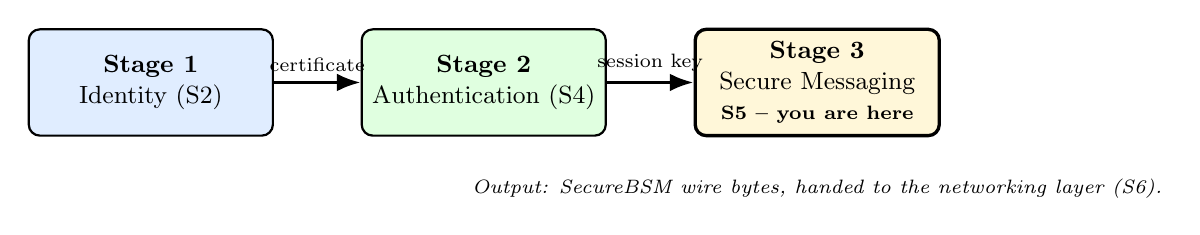
\begin{tikzpicture}[node distance=9mm and 11mm,every node/.style={font=\small},
    stage/.style={draw,rounded corners,minimum width=3.1cm,minimum height=1.35cm,
                  align=center,thick}]
  \node[stage,fill=boxblue]   (id)   {\textbf{Stage 1}\\Identity (S2)};
  \node[stage,fill=green!12,right=of id]   (auth) {\textbf{Stage 2}\\Authentication (S4)};
  \node[stage,fill=boxyellow,very thick,right=of auth] (msg)
       {\textbf{Stage 3}\\Secure Messaging\\\scriptsize \textbf{S5 -- you are here}};
  \draw[-{Latex[length=3mm]},very thick] (id)   -- (auth)
       node[midway,above,font=\scriptsize]{certificate};
  \draw[-{Latex[length=3mm]},very thick] (auth) -- (msg)
       node[midway,above,font=\scriptsize]{session key};
  \node[below=4mm of msg,font=\scriptsize\itshape,align=center]
       {Output: SecureBSM wire bytes, handed to the networking layer (S6).};
\end{tikzpicture}
\end{center}

% =====================================================================
\section{The Theory You Must Study}
% =====================================================================

\subsection{The Basic Safety Message (BSM)}
\textbf{Plain definition.} A BSM is the small data record a vehicle broadcasts:
its speed, heading, position, braking state and so on. In code it is the
\texttt{BasicSafetyMessage} dataclass.

\textbf{Real-life analogy.} A quick spoken status update: ``This is car A, doing
80, heading north-east, not braking, message number 5.''

\textbf{Why it exists.} Other cars need a small, standard, frequently-updated
record of what each nearby vehicle is doing, so they can react to danger.

\textbf{How it works here.} The dataclass carries nine fields:
\texttt{vehicle\_id}, \texttt{speed\_kmh}, \texttt{heading\_deg} (0 = North,
90 = East), \texttt{latitude}, \texttt{longitude}, \texttt{timestamp},
\texttt{sequence\_num}, \texttt{brake\_applied}, and \texttt{acceleration}.
Real V2V broadcasts a BSM about ten times a second; this project sends one per
second --- a deliberate slowdown so a human can watch the dashboard.

\textbf{Security property it relates to.} The BSM is the \emph{thing being
protected}; the rest of S5 is the protection.

\subsection{Sign-then-Encrypt}
\textbf{Plain definition.} ``Sign-then-Encrypt'' means: first create a digital
signature over the \emph{plaintext} message, then encrypt the message
\emph{and} its signature together.

\textbf{Real-life analogy.} You sign a letter by hand, then put the signed letter
inside a sealed, tamper-evident envelope. Anyone who opens the envelope finds a
letter that already carries your signature.

\textbf{Why it exists --- the alternative is worse.} The opposite order,
Encrypt-then-Sign, signs the \emph{ciphertext}. An attacker could then peel that
signature off and glue it onto a \emph{different} ciphertext, because the
signature was never tied to the actual message content. By signing the plaintext
first, the signature is bound to what the message really says. The file's own
docstring states this reasoning explicitly.

\textbf{How it works here.} \texttt{secure\_send} runs: serialize BSM
$\rightarrow$ \texttt{ecdsa\_sign} the BSM bytes $\rightarrow$ glue
\texttt{[length][BSM][signature]} together $\rightarrow$ \texttt{aes\_gcm\_encrypt}
the whole thing.

\textbf{Security property it provides.} \textbf{Non-repudiation} and
\textbf{authentication} (from the signature) wrapped inside
\textbf{confidentiality} and \textbf{integrity} (from the encryption).

\subsection{ECDSA Digital Signatures (recap from S3)}
A digital signature is a value made with a vehicle's \emph{private} key that
anyone with its \emph{public} key can verify. It proves \emph{who} wrote the
message and that it has not changed --- and because only the owner could sign,
they cannot later deny it. S5 simply calls \texttt{ecdsa\_sign} when sending and
\texttt{ecdsa\_verify} when receiving. \emph{Security property:}
\textbf{non-repudiation}, \textbf{authentication}, \textbf{integrity}.

\subsection{AES-256-GCM Authenticated Encryption (recap from S3)}
AES-256-GCM both hides the message (confidentiality) and attaches a 16-byte
authentication tag that detects any change (integrity). S5 calls
\texttt{aes\_gcm\_encrypt} when sending and \texttt{aes\_gcm\_decrypt} when
receiving; a tampered packet makes decryption fail. \emph{Security property:}
\textbf{confidentiality}, \textbf{integrity}.

\subsection{Serialization: JSON and Binary Packing}
\textbf{Plain definition.} \emph{Serialization} turns a structured object into a
flat sequence of bytes. S5 uses \emph{two} kinds:
\begin{itemize}
  \item \textbf{JSON} (JavaScript Object Notation) --- a human-readable text
        format. The BSM fields are turned into JSON text, then into bytes
        (\texttt{to\_bytes} uses \texttt{json.dumps}).
  \item \textbf{Binary struct packing} --- a compact fixed-layout byte format,
        used for the outer \texttt{SecureBSM} envelope.
\end{itemize}

\textbf{Real-life analogy.} JSON is filling in a paper form with words you can
read. Binary packing is a barcode: dense, exact, not human-readable, but quick
and unambiguous for a machine.

\textbf{Why two formats?} The BSM \emph{content} benefits from JSON's
flexibility. The outer envelope needs an exact, compact layout so the receiver
can find each field at a known position --- JSON would be wasteful and harder to
parse byte-precisely.

\textbf{Security property it provides.} None directly --- it is about format.

\subsection{Length-Prefixing and Big-Endian (the \texttt{struct} module)}
\textbf{Plain definition.} \emph{Length-prefixing} means writing a field's length
\emph{just before} the field itself, so the reader knows exactly how many bytes
to take. \emph{Big-endian} is the convention of writing the most significant byte
first (the ``natural'' left-to-right order for numbers).

\textbf{Real-life analogy.} A parcel label that says ``contents: 1742 grams''
before you open it --- you know what to expect. Big-endian is writing the number
``one thousand'' as \texttt{1000}, not \texttt{0001}.

\textbf{Why it exists.} Variable-length fields (the sender's name, the
ciphertext) have no fixed size. Without a length written in front, the receiver
cannot tell where one field ends and the next begins.

\textbf{How it works here.} The \texttt{struct} module packs numbers into bytes:
\texttt{struct.pack(">H", n)} writes \texttt{n} as a 2-byte big-endian unsigned
integer (\texttt{">"} = big-endian, \texttt{"H"} = 2-byte), and
\texttt{struct.pack(">I", n)} writes a 4-byte one (\texttt{"I"} = 4-byte).
\texttt{struct.unpack\_from} reads them back at a given offset.

\textbf{Security property it provides.} None directly --- but \emph{reliable}
framing avoids parsing errors that could be abused.

\subsection{Sequence Numbers and Replay Defence}
\textbf{Plain definition.} A \emph{sequence number} is a counter that increases
by one with every message a vehicle sends. The receiver remembers the last
number it saw and rejects anything not strictly greater.

\textbf{Real-life analogy.} Numbered tickets at a deli counter. If you are
holding ticket 8 and someone hands you ticket 5 again, you know it is an old,
re-used ticket.

\textbf{Why it exists.} A replayed message carries an \emph{old} sequence number.
A suppressed-and-delayed message arrives out of order. Requiring the number to
always increase catches both --- a replayed or stale BSM has a number less than
or equal to the last accepted one.

\textbf{How it works here.} \texttt{secure\_receive} takes a \texttt{last\_seq}
argument; if the new BSM's \texttt{sequence\_num} is \texttt{<= last\_seq} it
raises \texttt{SequenceError}. Combined with the 5-second timestamp window
(\texttt{TimestampValidator}, from S4), an old message has two ways to be caught.

\textbf{Honest note.} \texttt{secure\_receive} also \emph{accepts} a
\texttt{replay\_cache} argument, but --- unlike the handshake --- it does
\emph{not} actually consult the nonce cache in its body. For BSMs the replay
defence is the \emph{sequence number} plus the \emph{timestamp window}, not the
nonce cache. This is worth stating plainly if an examiner asks.

\textbf{Security property it provides.} \textbf{Replay prevention}.

% =====================================================================
\section{Code Walkthrough}
% =====================================================================

\texttt{v2v\_protocol.py} contains: three exceptions, two dataclasses
(\texttt{BasicSafetyMessage}, \texttt{SecureBSM}), the \texttt{MessageLogger}
class, and the two key functions \texttt{secure\_send} and
\texttt{secure\_receive}.

\subsection{The three exceptions}
\begin{lstlisting}[style=py,caption={v2v\_protocol.py --- the messaging exceptions.}]
class TamperError(Exception):
    """Message was modified in transit (AES-GCM tag mismatch or bad sig)."""

class ReplayError(Exception):
    """Duplicate message detected (same nonce or old timestamp)."""

class SequenceError(Exception):
    """Sequence number out of order -- possible message suppression."""
\end{lstlisting}
\textbf{Explanation:} \texttt{TamperError} means the packet failed an integrity
check (the AES-GCM tag or the ECDSA signature). \texttt{SequenceError} means the
sequence number went backwards. \texttt{ReplayError} is defined for completeness.
Naming each makes the dashboard's alert log precise.

\subsection{BasicSafetyMessage --- the plain message}
\begin{lstlisting}[style=py,caption={v2v\_protocol.py --- the BasicSafetyMessage dataclass.}]
@dataclass
class BasicSafetyMessage:
    vehicle_id: str
    speed_kmh: float
    heading_deg: float       # 0 = North, 90 = East
    latitude: float
    longitude: float
    timestamp: float
    sequence_num: int
    brake_applied: bool
    acceleration: float = 0.0

    def to_bytes(self) -> bytes:
        return json.dumps(asdict(self)).encode("utf-8")

    @classmethod
    def from_bytes(cls, data: bytes) -> BasicSafetyMessage:
        return cls(**json.loads(data.decode("utf-8")))
\end{lstlisting}
\textbf{Step by step:}
\begin{enumerate}
  \item The nine fields hold everything one safety broadcast says.
  \item \texttt{to\_bytes}: \texttt{asdict(self)} turns the object into a plain
        dictionary; \texttt{json.dumps} turns that into JSON text;
        \texttt{.encode("utf-8")} turns the text into bytes ready to be signed
        and encrypted.
  \item \texttt{from\_bytes}: the reverse --- decode bytes to text, parse the
        JSON to a dictionary, and build a fresh \texttt{BasicSafetyMessage}.
\end{enumerate}
\textbf{Theory link:} JSON serialization. \emph{Analogy:} filling in the paper
form (\texttt{to\_bytes}) and reading it back (\texttt{from\_bytes}).

\subsection{SecureBSM --- the on-the-wire envelope}
\begin{lstlisting}[style=py,caption={v2v\_protocol.py --- SecureBSM and its binary wire format.}]
@dataclass
class SecureBSM:
    ciphertext: bytes
    nonce: bytes          # 12-byte AES-GCM nonce
    auth_tag: bytes       # 16-byte AES-GCM tag
    sender_id: str
    sequence_num: int

    def to_bytes(self) -> bytes:
        # Wire format:
        # [sid_len:2][sid][seq:4][nonce:12][tag:16][ct_len:4][ciphertext]
        sid = self.sender_id.encode("utf-8")
        parts = [
            struct.pack(">H", len(sid)),
            sid,
            struct.pack(">I", self.sequence_num),
            self.nonce,    # always 12 bytes
            self.auth_tag, # always 16 bytes
            struct.pack(">I", len(self.ciphertext)),
            self.ciphertext,
        ]
        return b"".join(parts)

    @classmethod
    def from_bytes(cls, data: bytes) -> SecureBSM:
        offset = 0
        sid_len = struct.unpack_from(">H", data, offset)[0]; offset += 2
        sender_id = data[offset:offset + sid_len].decode("utf-8"); offset += sid_len
        seq = struct.unpack_from(">I", data, offset)[0]; offset += 4
        nonce = data[offset:offset + 12]; offset += 12
        tag = data[offset:offset + 16]; offset += 16
        ct_len = struct.unpack_from(">I", data, offset)[0]; offset += 4
        ciphertext = data[offset:offset + ct_len]
        return cls(ciphertext, nonce, tag, sender_id, seq)
\end{lstlisting}
\textbf{Step by step (\texttt{to\_bytes}):}
\begin{enumerate}
  \item Encode the sender's name to bytes.
  \item Write its length as a 2-byte big-endian number (\texttt{">H"}), then the
        name itself --- length-prefixing in action.
  \item Write the sequence number as a 4-byte big-endian number (\texttt{">I"}).
  \item Append the nonce (always 12 bytes) and the auth tag (always 16 bytes) ---
        no length prefix needed because their sizes are fixed.
  \item Write the ciphertext length (4 bytes), then the ciphertext.
  \item \texttt{b"".join(parts)} concatenates everything into one byte string.
\end{enumerate}
\textbf{\texttt{from\_bytes}} walks an \texttt{offset} cursor through the bytes,
reading each field at its known position --- the exact reverse of
\texttt{to\_bytes}. \textbf{Theory link:} binary serialization, length-prefixing,
big-endian. \emph{Analogy:} packing a parcel with a clear packing list, then
unpacking it item by item.

\subsection{MessageLogger --- the record keeper}
\textbf{Purpose:} keep a rolling record of sent/received messages and security
alerts, plus counters, for the dashboard (S7) to display.
\begin{lstlisting}[style=py,caption={v2v\_protocol.py --- MessageLogger (key parts).}]
class MessageLogger:
    def __init__(self, max_messages: int = 50) -> None:
        self._messages: list[dict] = []
        self._alerts: list[dict] = []
        self._max = max_messages
        self.total_sent = 0
        self.total_received = 0
        self.tamper_blocked = 0
        self.replay_blocked = 0

    def log_sent(self, bsm): ...        # +1 total_sent, append a SENT entry
    def log_received(self, bsm, security_props): ...   # +1 total_received
    def log_alert(self, alert_type, details):
        if alert_type == "TAMPER":  self.tamper_blocked += 1
        elif alert_type == "REPLAY": self.replay_blocked += 1
        self._alerts.append({...})
\end{lstlisting}
\textbf{Step by step:}
\begin{enumerate}
  \item It holds two rolling lists --- \texttt{\_messages} and \texttt{\_alerts}
        --- and four counters.
  \item \texttt{log\_sent} / \texttt{log\_received} append a small dictionary
        describing the message and trim the list to \texttt{max\_messages}
        (default 50) so memory does not grow forever.
  \item \texttt{log\_alert} bumps \texttt{tamper\_blocked} or
        \texttt{replay\_blocked} depending on the alert type, and records the
        alert with a timestamp.
  \item \texttt{get\_recent}, \texttt{get\_alerts} and \texttt{clear\_alerts} are
        read/clear helpers the dashboard calls.
\end{enumerate}
\textbf{Theory link:} this is \emph{observability}, not a defence --- it lets a
human \emph{see} that the defences fired. \emph{Analogy:} the CCTV logbook at a
building's front desk.

\subsection{secure\_send() --- Sign-then-Encrypt}
\begin{lstlisting}[style=py,caption={v2v\_protocol.py --- secure\_send: the sending pipeline.}]
def secure_send(bsm, session_key, signing_key, logger) -> bytes:
    # Step 1: serialize BSM to bytes
    bsm_bytes = bsm.to_bytes()
    # Step 2: sign the PLAINTEXT (Sign-then-Encrypt)
    signature = ecdsa_sign(signing_key, bsm_bytes)
    # Step 3: combine with a 4-byte length prefix
    payload = struct.pack(">I", len(bsm_bytes)) + bsm_bytes + signature
    # Step 4: AES-256-GCM encrypt -- confidentiality + integrity
    ciphertext, nonce, auth_tag = aes_gcm_encrypt(session_key, payload)
    # Step 5: wrap in SecureBSM and return wire bytes
    secure = SecureBSM(ciphertext, nonce, auth_tag, bsm.vehicle_id, bsm.sequence_num)
    logger.log_sent(bsm)
    return secure.to_bytes()
\end{lstlisting}
\textbf{Step by step:}
\begin{enumerate}
  \item \textbf{Serialize} --- turn the BSM into JSON bytes.
  \item \textbf{Sign the plaintext} --- \texttt{ecdsa\_sign} produces a signature
        over those exact bytes. Doing this \emph{before} encryption is the whole
        point of Sign-then-Encrypt.
  \item \textbf{Combine} --- glue \texttt{[4-byte length][BSM bytes][signature]}
        so the receiver can later split them apart again.
  \item \textbf{Encrypt} --- \texttt{aes\_gcm\_encrypt} encrypts the combined
        payload, returning ciphertext, a fresh nonce, and a 16-byte tag.
  \item \textbf{Wrap} --- build a \texttt{SecureBSM}, log the send, and return
        \texttt{secure.to\_bytes()} --- the final wire bytes.
\end{enumerate}
\textbf{Arguments:} \texttt{bsm} (the message), \texttt{session\_key} (32-byte
AES key from the handshake), \texttt{signing\_key} (this vehicle's ECDSA private
key), \texttt{logger}. \textbf{Returns:} wire-format \texttt{bytes}.
\textbf{Theory link:} Sign-then-Encrypt; ECDSA; AES-GCM; length-prefixing.

\subsection{secure\_receive() --- Decrypt-then-Verify}
\begin{lstlisting}[style=py,caption={v2v\_protocol.py --- secure\_receive: the receiving pipeline.}]
def secure_receive(data, session_key, peer_verify_key, replay_cache,
                   timestamp_validator, logger, last_seq=None):
    # Step 1: parse SecureBSM from raw bytes
    secure = SecureBSM.from_bytes(data)
    # Step 2: AES-GCM decrypt -- 1 changed bit -> failure
    try:
        plaintext = aes_gcm_decrypt(session_key, secure.ciphertext,
                                    secure.nonce, secure.auth_tag)
    except DecryptionError as exc:
        logger.log_alert("TAMPER", f"AES-GCM decryption failed: {exc}")
        raise TamperError("Message tampered -- AES-GCM auth tag mismatch") from exc
    # Step 3: split plaintext into BSM bytes + signature
    bsm_len = struct.unpack_from(">I", plaintext, 0)[0]
    bsm_bytes = plaintext[4:4 + bsm_len]
    signature = plaintext[4 + bsm_len:]
    # Step 4: verify the ECDSA signature
    if not ecdsa_verify(peer_verify_key, bsm_bytes, signature):
        logger.log_alert("TAMPER", "ECDSA signature verification failed")
        raise TamperError("Invalid ECDSA signature -- message not authentic")
    # Step 5: parse BSM, check sequence number, validate timestamp
    bsm = BasicSafetyMessage.from_bytes(bsm_bytes)
    if last_seq is not None and bsm.sequence_num <= last_seq:
        logger.log_alert("REPLAY", f"Seq {bsm.sequence_num} <= last {last_seq}")
        raise SequenceError(f"Sequence {bsm.sequence_num} not greater than {last_seq}")
    timestamp_validator.validate(bsm.timestamp)
    logger.log_received(bsm, {"authenticated": True, "encrypted": True,
                              "integrity_verified": True, "replay_protected": True})
    return bsm
\end{lstlisting}
\textbf{Step by step:}
\begin{enumerate}
  \item \textbf{Parse} the raw bytes back into a \texttt{SecureBSM}
        (\texttt{from\_bytes}).
  \item \textbf{Decrypt} with \texttt{aes\_gcm\_decrypt}. If a single bit was
        changed, the tag check fails: the code catches \texttt{DecryptionError},
        logs a \texttt{TAMPER} alert, and raises \texttt{TamperError}.
  \item \textbf{Split} the decrypted payload using the 4-byte length prefix into
        the BSM bytes and the signature.
  \item \textbf{Verify the signature} with \texttt{ecdsa\_verify} against the
        peer's public key. If it fails, log a \texttt{TAMPER} alert and raise
        \texttt{TamperError}. This is the second integrity check --- and the one
        that gives \textbf{non-repudiation}.
  \item \textbf{Parse and validate.} Rebuild the BSM. If the sequence number is
        not greater than \texttt{last\_seq}, raise \texttt{SequenceError}
        (replay). Then \texttt{timestamp\_validator.validate} rejects a stale
        timestamp. If all pass, log a successful receive and return the BSM.
\end{enumerate}
\textbf{Arguments / return / exceptions:} returns the verified
\texttt{BasicSafetyMessage}; raises \texttt{TamperError} (bad tag or bad
signature), \texttt{SequenceError} (replay), or \texttt{StaleMessageError}
(stale timestamp). \textbf{Honest note:} the \texttt{replay\_cache} parameter is
accepted but not used in the body --- BSM replay defence here is the sequence
number and timestamp. \textbf{Theory link:} AES-GCM integrity, ECDSA
authentication, sequence/timestamp replay defence.

\subsection{The demo block}
The \texttt{if \_\_name\_\_ == "\_\_main\_\_"} block builds a session key, creates
a BSM, calls \texttt{secure\_send} then \texttt{secure\_receive} (showing a clean
round-trip), then flips a byte and shows the tampered message is rejected with a
\texttt{TamperError}. We run it next.

% =====================================================================
\section{Hands-On / Practical}
% =====================================================================

\subsection{Run the messaging protocol by itself}
\texttt{v2v\_protocol.py} needs no certificates and no network --- run it directly:
\begin{lstlisting}[style=term]
python protocol\v2v_protocol.py
\end{lstlisting}

\noindent\textbf{Expected output (sample):}
\begin{lstlisting}[style=term]
=== V2V MESSAGE PROTOCOL DEMO ===

Session key: 4a9c1f0b7e2d6688c3a5...

[SEND] BSM: speed=72.5 km/h, seq=1
[WIRE] 338 bytes on the wire (encrypted)
[RECV] BSM: speed=72.5 km/h, seq=1
[OK] All security checks passed!

--- TAMPER TEST ---
[OK] Tampered message REJECTED: Message tampered -- AES-GCM auth tag mismatch

Stats: sent=1, recv=1, tamper_blocked=1
\end{lstlisting}

\subsection{What the output lines mean}
\begin{itemize}
  \item \texttt{Session key} --- a 32-byte key (here simulated, normally from the
        S4 handshake).
  \item \texttt{[SEND]} --- the plain BSM before protection.
  \item \texttt{[WIRE] 338 bytes} --- the size of the signed-and-encrypted
        packet; the exact number depends on the JSON content.
  \item \texttt{[RECV] ... [OK]} --- decryption, signature check, sequence and
        timestamp checks all passed; the message came back identical.
  \item \texttt{Tampered message REJECTED} --- one flipped byte made the AES-GCM
        tag mismatch, so \texttt{secure\_receive} raised \texttt{TamperError}.
  \item \texttt{tamper\_blocked=1} --- the \texttt{MessageLogger} counted the
        blocked attack.
\end{itemize}

\subsection{Try This Yourself (mini-experiment)}
In the demo's tamper test, the line \texttt{tampered[len(tampered) // 2] \^{}= 0xFF}
flips one byte in the \emph{middle} of the packet. Change it to flip a byte near
the \emph{start} instead:
\begin{lstlisting}[style=term]
tampered[0] ^= 0xFF        # flip the very first byte
\end{lstlisting}
\textbf{Predict before you run.} Byte~0 is part of the \texttt{sid\_len} field
(the 2-byte sender-name length). Corrupting it makes \texttt{SecureBSM.from\_bytes}
read a wrong length and the unpacking fails \emph{before} decryption even starts
--- so instead of a clean \texttt{TamperError} you may see a different exception
(for example a \texttt{struct} or decode error), caught by the demo's general
\texttt{except Exception} branch as ``Message rejected''. Lesson: tampering is
caught \emph{somewhere} on every path --- but exactly which check fires depends
on \emph{which} bytes you damage.

% =====================================================================
\section{Attack Relevance}
% =====================================================================

S5 is the layer that defends \emph{every individual safety message}. It is
exercised directly by \texttt{attacks/tamper\_attack.py} and
\texttt{attacks/replay\_attack.py}.

\begin{table}[h]
\centering
\small
\begin{tabular}{@{}p{2.5cm} p{6.1cm} p{4.9cm}@{}}
\toprule
\textbf{Attack} & \textbf{How S5 stops it} & \textbf{The mechanism}\\
\midrule
Tamper & A changed byte breaks the AES-GCM tag; a forged body breaks the ECDSA
signature. & \texttt{aes\_gcm\_decrypt} / \texttt{ecdsa\_verify} $\to$
\texttt{TamperError}.\\
Replay & A re-sent BSM carries an old sequence number or a stale timestamp. &
sequence check $\to$ \texttt{SequenceError}; \texttt{TimestampValidator} $\to$
\texttt{StaleMessageError}.\\
Eavesdrop & The BSM travels as AES-256 ciphertext; unreadable without the
session key. & \texttt{aes\_gcm\_encrypt} in \texttt{secure\_send}.\\
Forgery / denial & The plaintext signature ties the message to its true author,
who cannot deny it. & ECDSA signature (non-repudiation).\\
\bottomrule
\end{tabular}
\caption{S5 defends confidentiality, integrity, replay prevention and non-repudiation per message.}
\end{table}

\noindent\textbf{Why Sign-then-Encrypt matters for the attacker.} Because the
signature covers the \emph{plaintext}, an attacker cannot take a valid signature
from one message and re-attach it to a different one --- the signature would not
match the new content. And because the signature is \emph{inside} the encrypted
envelope, the attacker cannot even read or strip it without the session key.
\textbf{Honest scope note:} S5 protects each message, but it relies on a correct
session key from S4; if the handshake were skipped or compromised, S5 alone could
not help.

% =====================================================================
\section{Illustrations}
% =====================================================================

\subsection{Diagram 1 --- the Sign-then-Encrypt pipeline}
\begin{center}
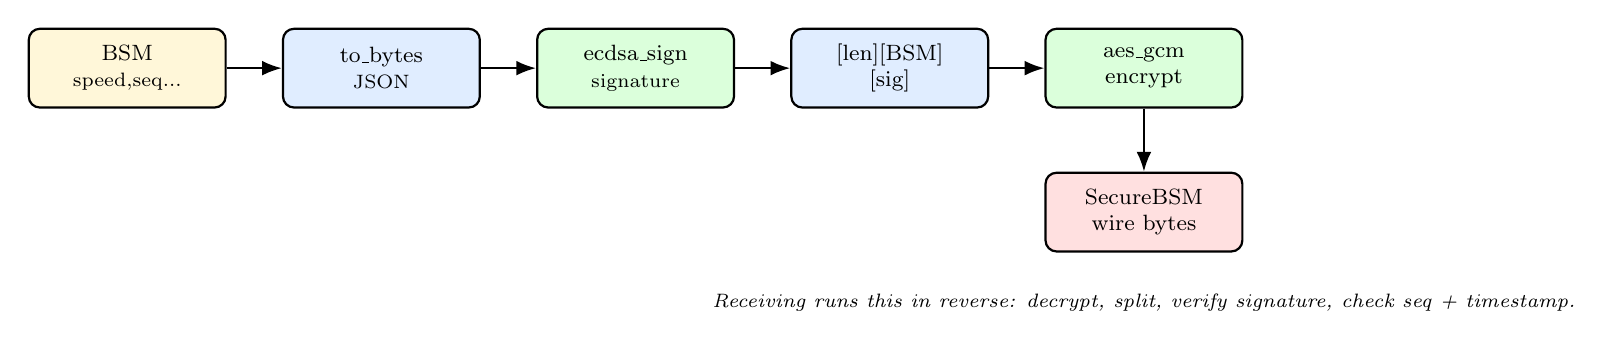
\begin{tikzpicture}[font=\footnotesize,node distance=5mm,
   box/.style={draw,thick,rounded corners,minimum width=2.5cm,minimum height=1.0cm,
               align=center}]
  \node[box,fill=boxyellow] (bsm) {BSM\\\scriptsize speed,seq...};
  \node[box,fill=boxblue,right=7mm of bsm] (json) {to\_bytes\\\scriptsize JSON};
  \node[box,fill=green!14,right=7mm of json] (sign) {ecdsa\_sign\\\scriptsize signature};
  \node[box,fill=boxblue,right=7mm of sign] (comb) {[len][BSM]\\{[sig]}};
  \node[box,fill=green!14,right=7mm of comb] (enc) {aes\_gcm\\encrypt};
  \node[box,fill=red!12,below=8mm of enc] (wire) {SecureBSM\\wire bytes};
  \draw[-{Latex[length=2.5mm]},thick] (bsm) -- (json);
  \draw[-{Latex[length=2.5mm]},thick] (json) -- (sign);
  \draw[-{Latex[length=2.5mm]},thick] (sign) -- (comb);
  \draw[-{Latex[length=2.5mm]},thick] (comb) -- (enc);
  \draw[-{Latex[length=2.5mm]},thick] (enc) -- (wire);
  \node[below=4mm of wire,font=\scriptsize\itshape]
       {Receiving runs this in reverse: decrypt, split, verify signature, check seq + timestamp.};
\end{tikzpicture}
\end{center}

\subsection{Diagram 2 --- the SecureBSM wire format}
\begin{center}
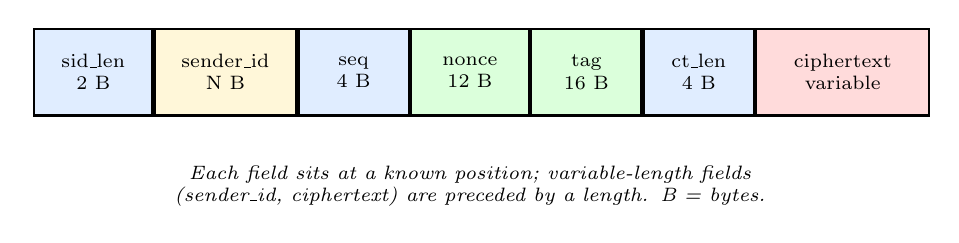
\begin{tikzpicture}[font=\scriptsize,
   f/.style={draw,thick,minimum height=1.1cm,align=center}]
  \node[f,fill=boxblue,minimum width=1.5cm]              (a) {sid\_len\\2 B};
  \node[f,fill=boxyellow,minimum width=1.8cm,right=0 of a] (b) {sender\_id\\N B};
  \node[f,fill=boxblue,minimum width=1.4cm,right=0 of b] (c) {seq\\4 B};
  \node[f,fill=green!14,minimum width=1.5cm,right=0 of c] (d) {nonce\\12 B};
  \node[f,fill=green!14,minimum width=1.4cm,right=0 of d] (e) {tag\\16 B};
  \node[f,fill=boxblue,minimum width=1.4cm,right=0 of e] (g) {ct\_len\\4 B};
  \node[f,fill=red!14,minimum width=2.2cm,right=0 of g] (h) {ciphertext\\variable};
  \node[below=5mm of d,font=\scriptsize\itshape,align=center,text width=11cm]
       {Each field sits at a known position; variable-length fields
        (sender\_id, ciphertext) are preceded by a length. B = bytes.};
\end{tikzpicture}
\end{center}

% =====================================================================
\section{Presentation Pack}
% =====================================================================

\subsection{Slide Outline}

\textbf{Slide 1 --- The Job of S5.}
\begin{itemize}
  \item The handshake gave us a shared key --- now we can talk.
  \item A BSM is a tiny ``speed, heading, braking'' status message.
  \item S5 turns a plain BSM into a safe packet, and back again.
  \item One file: \texttt{v2v\_protocol.py}.
\end{itemize}

\textbf{Slide 2 --- Sign-then-Encrypt.}
\begin{itemize}
  \item First sign the plaintext, then encrypt message + signature together.
  \item Sign first $\to$ the signature is tied to the real content.
  \item Encrypt-then-Sign would let an attacker swap signatures.
  \item Result: a signed letter inside a sealed envelope.
\end{itemize}

\textbf{Slide 3 --- The SecureBSM Wire Format.}
\begin{itemize}
  \item An exact byte layout: lengths, ids, nonce, tag, ciphertext.
  \item Length-prefixing tells the receiver where each field ends.
  \item Big-endian packing via Python's \texttt{struct} module.
  \item Fixed-size fields (nonce 12 B, tag 16 B) need no length.
\end{itemize}

\textbf{Slide 4 --- Receiving: Four Checks.}
\begin{itemize}
  \item Decrypt --- AES-GCM tag catches any tampering.
  \item Verify signature --- ECDSA proves the true author.
  \item Sequence number --- must always increase (anti-replay).
  \item Timestamp --- must be within 5 seconds (anti-replay).
\end{itemize}

\textbf{Slide 5 --- What S5 Guarantees Per Message.}
\begin{itemize}
  \item Confidentiality + integrity (AES-256-GCM).
  \item Authentication + non-repudiation (ECDSA signature).
  \item Replay prevention (sequence + timestamp).
  \item A single flipped bit $\to$ \texttt{TamperError}.
\end{itemize}

\subsection{Speaker Talking Points (about 30--60 seconds each)}

\textbf{Slide 1.} ``After the handshake in the previous section, our two cars
share a secret key. Now they can actually talk. What they say are Basic Safety
Messages --- tiny records of speed, heading, position and braking. Section five
is the file that protects each of those messages. It takes a plain BSM, wraps it
in security, produces the exact bytes that go on the wire, and on the other side
unwraps it and checks it. It is all in one file, v2v\_protocol.py.''

\textbf{Slide 2.} ``The protection recipe is called Sign-then-Encrypt. We first
make a digital signature over the plain message, and only then encrypt the
message and its signature together. Order matters. If we encrypted first and
signed the ciphertext, an attacker could peel that signature off and stick it on
a different ciphertext, because the signature was never connected to the real
words. By signing the plaintext first, the signature is glued to what the
message actually says. Picture signing a letter by hand, then sealing it in a
tamper-evident envelope.''

\textbf{Slide 3.} ``A network only carries a flat stream of bytes, so we need an
exact layout --- the wire format. The SecureBSM packet is: a two-byte length,
then the sender's name, then a four-byte sequence number, then the twelve-byte
nonce, the sixteen-byte tag, a four-byte ciphertext length, and finally the
ciphertext. The trick is length-prefixing: before any variable-size field we
write its length, so the receiver knows exactly where it ends. We build this with
Python's struct module in big-endian order.''

\textbf{Slide 4.} ``Receiving is the reverse, and it is four checks in a row.
First we decrypt --- and AES-GCM's tag means any tampering makes decryption fail
outright. Second we verify the ECDSA signature, which proves the message really
came from the claimed car. Third we check the sequence number is larger than the
last one we accepted --- an old or replayed message has an old number. Fourth we
check the timestamp is fresh, within five seconds. Only a message that passes all
four is delivered.''

\textbf{Slide 5.} ``So per message, S5 delivers four security properties at once.
AES-256-GCM gives confidentiality and integrity. The ECDSA signature gives
authentication and non-repudiation --- the sender cannot deny it. And the
sequence number plus timestamp give replay prevention. The demo proves it: flip
a single bit anywhere in the packet and the receiver throws a TamperError instead
of trusting the message.''

\subsection{Live-Demo Script}
\begin{enumerate}
  \item \textbf{Run the demo.} Execute \texttt{python
        protocol\textbackslash v2v\_protocol.py}.
  \item \textbf{Point at the round-trip.} \texttt{[SEND]} then \texttt{[RECV]}
        with the same speed and sequence number --- ``protected and recovered
        perfectly.''
  \item \textbf{Point at the wire size.} \texttt{[WIRE] 338 bytes} --- ``that is
        the signed, encrypted packet.''
  \item \textbf{Point at the tamper test.} \texttt{Tampered message REJECTED} ---
        ``one byte changed, the whole message refused.''
  \item \textbf{Optional break-it.} Change the flipped index to \texttt{0} (see
        the mini-experiment) and show a different rejection path.
\end{enumerate}

\subsection{Examiner Q\&A}
\begin{enumerate}
  \item \textbf{Q: What is a BSM and what fields does it carry here?}\\
        A: A Basic Safety Message. The \texttt{BasicSafetyMessage} dataclass
        carries vehicle id, speed, heading, latitude, longitude, timestamp,
        sequence number, brake flag and acceleration.
  \item \textbf{Q: What is Sign-then-Encrypt and why not the reverse?}\\
        A: Sign the plaintext first, then encrypt message + signature. The
        reverse (signing the ciphertext) would let an attacker move a signature
        onto a different ciphertext, since it would not be bound to content.
  \item \textbf{Q: Describe the SecureBSM wire format.}\\
        A: \texttt{[sid\_len:2][sender\_id][seq:4][nonce:12][tag:16][ct\_len:4]
        [ciphertext]} --- length-prefixed, big-endian, built with \texttt{struct}.
  \item \textbf{Q: Why length-prefix the variable fields?}\\
        A: The sender name and ciphertext have no fixed size; writing the length
        first tells the receiver exactly how many bytes to read.
  \item \textbf{Q: How does \texttt{secure\_receive} detect a tampered message?}\\
        A: Two ways: \texttt{aes\_gcm\_decrypt} fails if the ciphertext/nonce/tag
        changed (\texttt{DecryptionError} $\to$ \texttt{TamperError}), and
        \texttt{ecdsa\_verify} fails if the body does not match the signature.
  \item \textbf{Q: How does S5 stop replay?}\\
        A: The sequence number must be strictly greater than the last accepted
        one (\texttt{SequenceError} otherwise), and the timestamp must be within
        5 seconds.
  \item \textbf{Q: The \texttt{replay\_cache} argument --- is it used?}\\
        A: It is accepted by \texttt{secure\_receive} but not consulted in the
        body. BSM replay defence is the sequence number plus the timestamp; the
        nonce cache is used by the handshake, not here.
  \item \textbf{Q: What does \texttt{MessageLogger} contribute to security?}\\
        A: Nothing directly --- it is observability. It records sent/received
        messages and counts blocked tamper/replay attempts so the dashboard can
        display them.
\end{enumerate}

% =====================================================================
\section{Glossary}
% =====================================================================
\begin{description}[style=nextline,leftmargin=0pt]
  \item[BSM] Basic Safety Message: the small status broadcast of a vehicle.
  \item[BasicSafetyMessage] The dataclass holding the BSM fields.
  \item[SecureBSM] The signed-and-encrypted on-the-wire form of a BSM.
  \item[Sign-then-Encrypt] Sign the plaintext, then encrypt message + signature.
  \item[Plaintext] The original readable message before encryption.
  \item[Ciphertext] The scrambled output of encryption.
  \item[Wire format] The exact byte layout of a packet sent over a network.
  \item[Serialization] Turning an object into a flat sequence of bytes.
  \item[JSON] A human-readable text format for structured data.
  \item[struct module] Python module that packs/unpacks numbers into bytes.
  \item[Length-prefixing] Writing a field's length just before the field.
  \item[Big-endian] Byte order with the most significant byte first.
  \item[Nonce] A one-time 12-byte value for AES-GCM encryption.
  \item[Authentication tag] The 16-byte AES-GCM value that detects tampering.
  \item[ECDSA] Elliptic Curve Digital Signature Algorithm.
  \item[Digital signature] A private-key value provable with the public key.
  \item[Sequence number] A per-sender counter that must always increase.
  \item[Timestamp] The recorded creation time, checked for freshness.
  \item[Session key] The shared 32-byte AES key from the handshake.
  \item[TamperError] Exception meaning a packet failed an integrity check.
  \item[SequenceError] Exception meaning the sequence number went backwards.
  \item[MessageLogger] Class that records messages and alerts for the dashboard.
  \item[Non-repudiation] A sender cannot later deny having sent a message.
  \item[Confidentiality] Only the intended recipient can read the message.
  \item[Integrity] Any change to the message is detected.
\end{description}

% =====================================================================
\section{References and Further Study}
% =====================================================================
\begin{itemize}
  \item \textbf{Python struct module documentation} ---
        \url{https://docs.python.org/3/library/struct.html}\\
        Read for: the format codes \texttt{">H"} and \texttt{">I"} used in the
        wire format.
  \item \textbf{Python json module documentation} ---
        \url{https://docs.python.org/3/library/json.html}\\
        Read for: \texttt{json.dumps} / \texttt{json.loads} used by the BSM.
  \item \textbf{Python dataclasses documentation} ---
        \url{https://docs.python.org/3/library/dataclasses.html}\\
        Read for: how \texttt{BasicSafetyMessage} and \texttt{SecureBSM} work.
  \item \textbf{SAE J2735 (Basic Safety Message standard)} ---
        \url{https://www.sae.org/standards/content/j2735_202309/}\\
        Read for: the real-world BSM this project is inspired by.
  \item \textbf{Authenticated encryption (Wikipedia)} ---
        \url{https://en.wikipedia.org/wiki/Authenticated_encryption}\\
        Read for: why AES-GCM gives confidentiality and integrity together.
  \item \textbf{Sign-then-encrypt discussion (Cryptography Stack Exchange)} ---
        \url{https://crypto.stackexchange.com/questions/5458/should-we-sign-then-encrypt-or-encrypt-then-sign}\\
        Read for: the trade-offs between signing and encrypting order.
  \item \textbf{Endianness (Wikipedia)} ---
        \url{https://en.wikipedia.org/wiki/Endianness}\\
        Read for: what big-endian byte order means.
  \item \textbf{Digital signature (Wikipedia)} ---
        \url{https://en.wikipedia.org/wiki/Digital_signature}\\
        Read for: authentication, integrity and non-repudiation.
  \item \textbf{Python cryptography --- AEAD docs} ---
        \url{https://cryptography.io/en/latest/hazmat/primitives/aead/}\\
        Read for: the AES-GCM functions S5 calls.
  \item \textbf{Replay attack (Wikipedia)} ---
        \url{https://en.wikipedia.org/wiki/Replay_attack}\\
        Read for: why sequence numbers and timestamps defeat replay.
\end{itemize}

\vfill
\begin{center}\footnotesize\itshape
End of Section S5. Next: S6 --- the Vehicle Node and TCP networking that carries
these SecureBSM bytes.
\end{center}

\end{document}
